\documentclass[aspectratio=43]{beamer}
\mode<presentation>{
\usetheme{Dresden}
\setbeamercovered{transparent}
\usecolortheme{lsc}
}

\mode<handout>{
  % tema simples para ser impresso
  %\usepackage[bar]{beamerthemetree}
  % Colocando um fundo cinza quando for gerar transparências para serem impressas
  % mais de uma transparência por página
  \beamertemplatesolidbackgroundcolor{black!5}
}

\usepackage{amsmath,amssymb}
\usepackage[brazil]{varioref}
\usepackage[spanish]{babel}
\usepackage[utf8]{inputenc}
%\usepackage[latin1]{inputenc}
\usepackage{graphicx}
\usepackage{listings}
\usepackage{url}
\usepackage{colortbl}

\beamertemplatetransparentcovereddynamic

\title[\textit{Cálculo de métricas del paisaje a partir del SIOSE: una propuesta escalable basada en PostgreSQL/PostGIS}]{\textbf{CÁLCULO DE MÉTRICAS DE PAISAJE A PARTIR DEL SIOSE: UNA PROPUESTA ESCALABLE BASADA EN POSTGRESQL/POSTGIS}}
\author[]{
  \textbf{\small{Andrea Rosado Abad}} \\
  \footnotesize{Directores: Raquel Montorio Llovería y Daniel Borini Alves}}
  \institute[]{
	\textit{\tiny{Máster Universitario en\\ Tecnologías de la Información Geográfica para la Ordenación del Territorio: SIG y Teledetección}}\\}

% Se comentar a linha abaixo, irá aparecer a data quando foi compilada a apresentação  
\date{\footnotesize{14 de Diciembre de 2017}}
	

%\pgfdeclareimage[height=2cm]{inf}{Figs/unizar_logo.png}

% pode-se colocar o LOGO assim
%\logo{\pgfuseimage{inf}}

\titlegraphic{
\includegraphics[height=0.4cm]{Figs/unizar}\hfill
\includegraphics[height=0.4cm]{Figs/geo_unizar}\hfill
\includegraphics[height=0.3cm]{Figs/ua_logo}\hfill
\includegraphics[height=0.5cm]{Figs/iig_ua}}

\setbeamertemplate{navigation symbols}{} 

%Para quitar la barra del título de la diapositiva
%\setbeamertemplate{frametitle}{}
%\setbeamertemplate{frametitleshade}{}
\setbeamerfont{caption}{size=\tiny}
\usepackage{multirow}
\usepackage{colortbl}
\usepackage{xcolor}
\usepackage{enumerate}
\usepackage{tikz}
\usepackage{amsmath,amssymb,latexsym}




%%%%%%%%%%%%%%%%%%%%%%%%%%%%%%%%%%%%%%%%%%%%%%%%%%%%%%%%%%%%%%%%%%%%%%%%%%%%%%%%%%%%%%%%%%%%%%%%%%%%%%%%%%%%%%%%%%%%%%%%%%%%%%%%%%%%%%%%%%%%%%%%%%%%%%%%%%%%%%%%%%  S L I D E S  %%%%%%%%%%%%%%%%%%%%%%%%%%%%%%%%%%%%%%%%%%%%%%%%%%%%%%%%%%%%%%%%%%%%%%%%%%%%%%%%%%%%%%%%%%%%%%%%%%%%%%%%%%%%%%%%%%%%%%%%%%%%%%%%%%%%%%%%%%%%%%%%%%%%%%%%%%%%%%%%%%%%%




\begin{document}

{
\setbeamertemplate{headline}{}
\begin{frame}
\titlepage
\end{frame}

\begin{frame}
\frametitle{\textbf{Índice general}}
\tableofcontents
\end{frame}
}

\section{Contexto}
	
\begin{frame}{Objetivos}

\begin{figure}
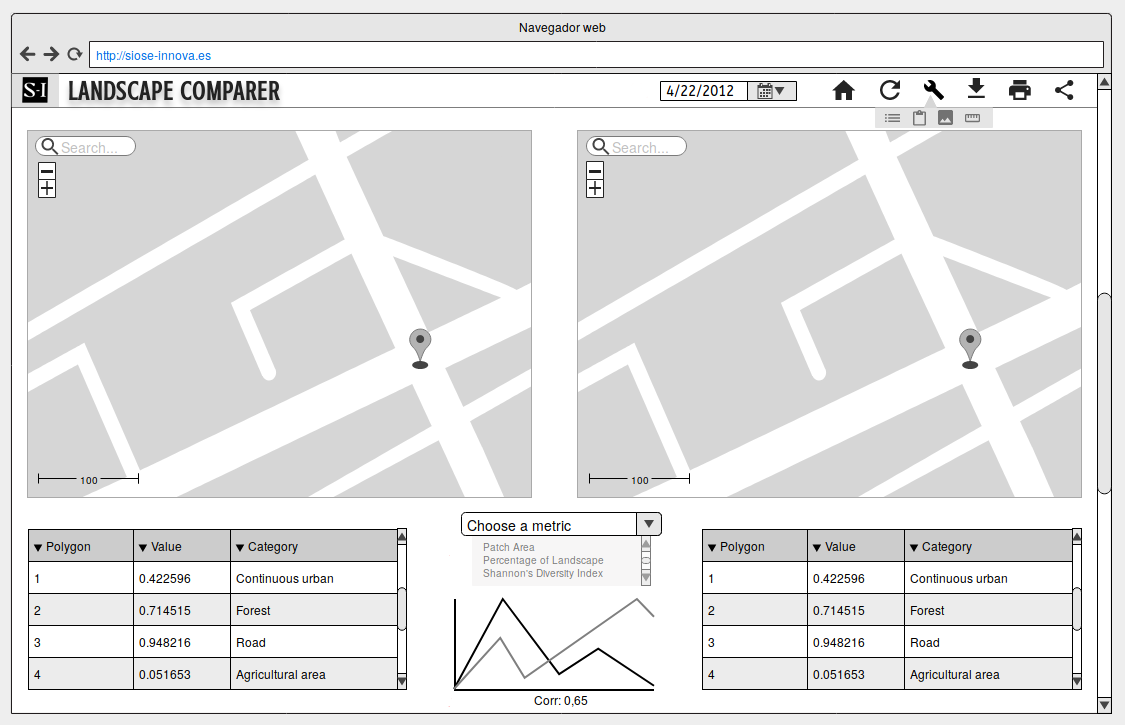
\includegraphics[height=6cm]{Prologo/Figs/visorweb} 
%\vspace{-1cm}
\caption{\textit{Prototipo de un visor cartográfico para el análisis (comparación) de la estructura del paisaje a partir del SIOSE.}}
\end{figure}


\end{frame}




\section{Introducción}
	
\section{Introducción}

\begin{frame}{El SIOSE}
\begin{itemize}
\item El SIOSE es una valiosa \textbf{base de datos de ocupación del suelo} que contiene un gran volumen de información territorial de toda España.
\item Desde su aparición en 2005, SIOSE se ha convertido en un repositorio de referencia para sus homólogos europeos, llegando a ser un \textbf{modelo para la iniciativa EAGLE} (\textit{SIOSE europeo}). 
\item A pesar de su gran potencial, el SIOSE presenta ciertos problemas de \textit{usabilidad} debidos a su gran volumen y complejidad.
\end{itemize}
\end{frame}

\begin{frame}{El SIOSE}
\begin{figure}
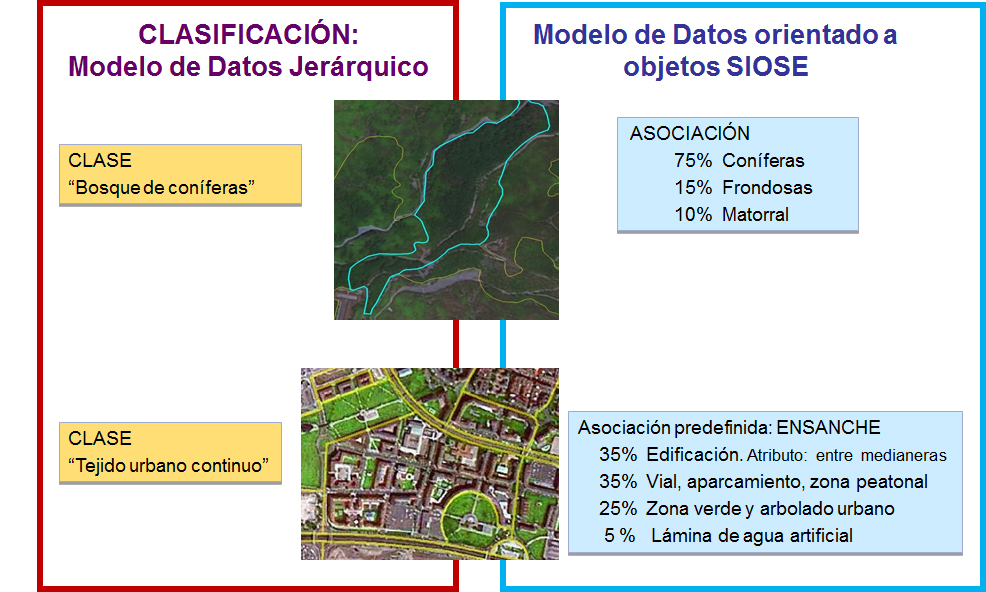
\includegraphics[width=\textwidth]{Introduccion/Figs/siose-oo.png}
\caption{Riqueza descriptiva del modelo de datos orientado a objetos del SIOSE frente a una clasificación jerárquica. Fuente: \url{www.siose.es}.\label{fig:siose-oo}}
\end{figure}
\end{frame}

\section{Objetivos}
	
\begin{frame}{Objetivos}
Objetivos
\end{frame}




\section{Metodología}
	
\begin{frame}{}
Metodologia
\end{frame}




\section{Resultados}
	
\begin{frame}{}
Resultados
\end{frame}




\section{Conclusiones y trabajo futuro}
	
\begin{frame}{}
Conclusiones
\end{frame}






{
\setbeamertemplate{headline}{}
\begin{frame}
\titlepage
\end{frame}

\end{document}
}

